% IPP
% Projekt - 1.
% Juraj Holub
% xholub40@stud.fit.vutbr.cz

\documentclass[a4paper, 10pt]{article}
\usepackage[utf8]{inputenc}
\usepackage[english]{babel}
\usepackage[T1]{fontenc}
\usepackage[left=2cm,top=2.5cm, right=2cm]{geometry}
\usepackage{hyperref}
\usepackage{graphicx}
\usepackage{float}

\title{Documentation to implementaition of task No. 1 to the IPP 2018/2019 }
\author{Name and surname: Juraj Holub\\ Login: xholub40}
\date{}

\begin{document}
	\maketitle
	\thispagestyle{empty}

% introduction
% proposal of solution
\section{Proposal of solution} \label{proposal}
Scheme of project solution is split to three blocks. 

First block split input string to tokens representation where one token represents atomic lexeme of input programming language IPPcode19. Token is implemented like data structure with two attributes. First attribute is identification of token, for example keywords or integer constant. Second attribute is value of token specified by his identification, for example integer constant contain specific integer value.

Second block is finite state machine (FSM). FSM input is string of tokens and machine verify lexical and syntactical correctness of input program.

Third and last block is generator of output in eXtensible Markup Language (XML). 

\begin{figure}[H] 
	\centering
	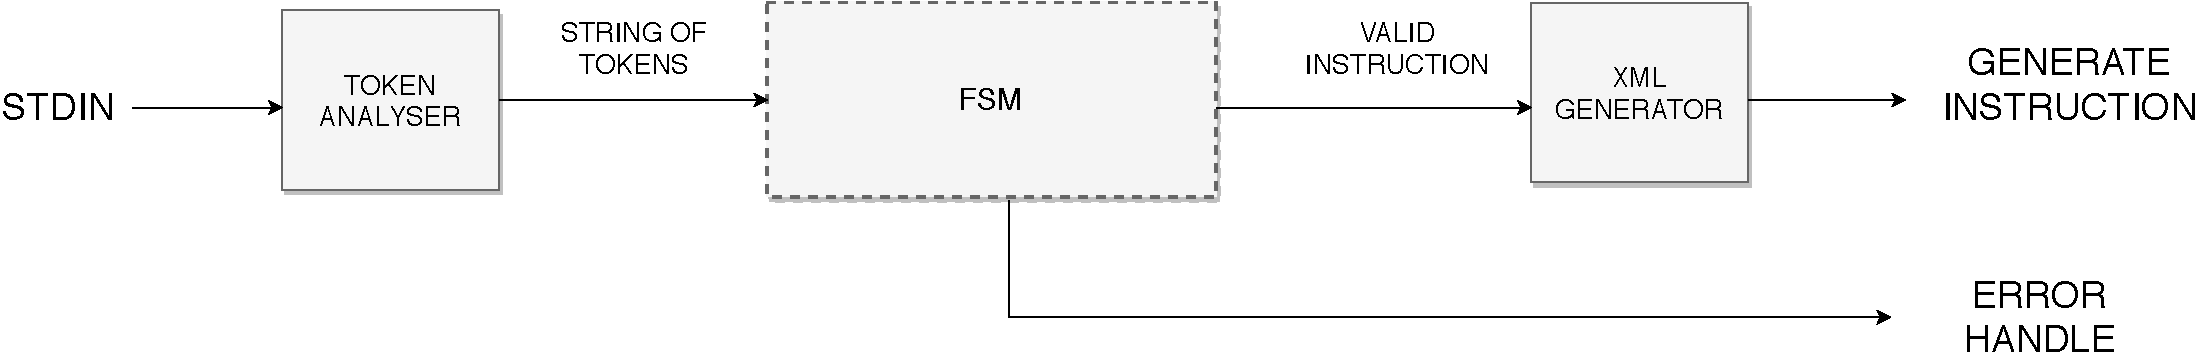
\includegraphics[width=.8 \paperwidth]{ipp_parse}
	\caption{Scheme of implemented parse solution.}
	\label{obr1}
\end{figure} 

Figure \ref{obr1} shows scheme of implemented algorithm of parsing IPPcode19 and generating XML output.

\section{Implementation details}
Suggested solution parted to three blocks described in section \ref{proposal} is implemented in three logical units:
\begin{itemize}
	\item \textbf{Tokens analyser}: Analyse input string from standard input of program char by char and convert them to the token representation. Supported tokens are instruction code, symbol, label, variable, type, white space, new line. Instruction codes are sorted to groups by number and types of arguments. Comments are ignored and token analyser skip them in input program string.
	\item \textbf{Parse}: Implementation of finite state machine. FSM input is actual token received from token analyser. Machine output depends on current state and current token whih lead to Mealy FSM. If input is valid then after every successive analyse of one IPPcode19 instruction is this instruction send to XML generator. Incorrect input lead to error state where FSM read rest of tokens and then inform about error.
	\item \textbf{XML generator}: Generate XML representation of IPPcode19. Input of class are one instruction with their arguments. Class implementation uses \href{http://php.net/manual/en/class.domdocument.php}{DOMDocument} library. This library is optimized for XML generating and brings advantages like converting XML key words inside of input data to correct representation. 
\end{itemize}


\end{document}
